\chapter{Linear and Logistic Regression}
%\begin{refsection}

\begin{figure}[h!]
\centering
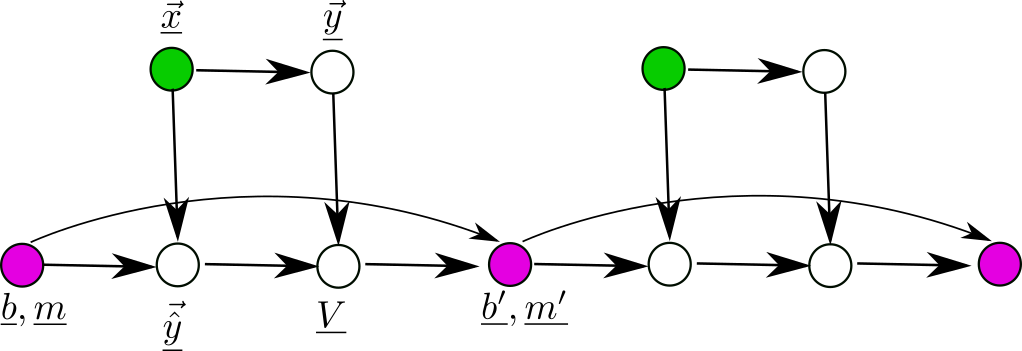
\includegraphics[width=5in]{linreg/linreg.png}
\caption{Linear Regression} 
\label{fig-linreg}
\end{figure}

\begin{figure}[h!]
\centering
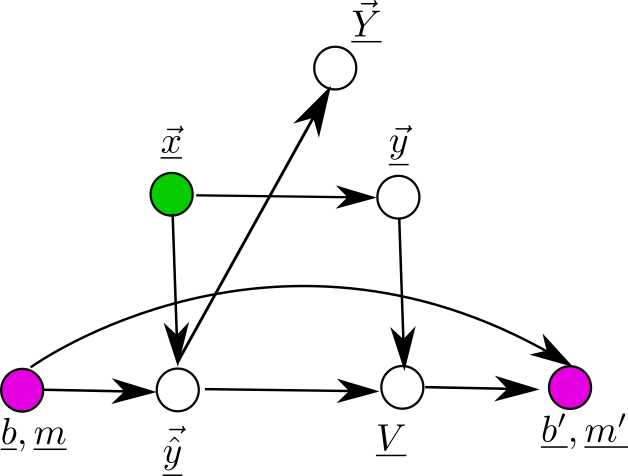
\includegraphics[width=3in]{linreg/linreg-emul.png}
\caption{Bnet of Fig.\ref{fig-linreg}  with new $\vec{\ul{Y}}$ node.}\label{fig-linreg-emul}
\end{figure}



Estimators $\hat{y}$ for linear and logistic regression.
\begin{itemize}
\item 

\textbf{Linear Regression:} $y\in \RR$. 
Note $\hat{y}\in \RR$. $(x,\hat{y}(x))$ is
the graph
of a straight line 
with y-intercept $b$ and slope $m$.
\beq
\hat{y}(x;b, m)= b + mx
\eeq

\item
\textbf{Logistic Regression:} $y\in\{0, 1\}$. Note $\hat{y}\in [0,1]$. $
(x,\hat{y}(x))$ is the graph
of a sigmoid.
 Often in literature, $b,m$ are replaced by $\beta_0, \beta_1$. 
\beq
\hat{y}(x;b, m)=\smoid(b + m x)
\eeq
\end{itemize}

Define
\beq
V(b, m)=\sum_{x,y}P(x,y)| y-\hat{y}(x;b, m)|^2
\;.\label{eq-norm-cost}
\eeq
We want to minimize $V(b,m)$ (called a cost or loss function) wrt $b$ and $m$.


Node TPMs of Bnet of Fig.\ref{fig-linreg}
given next in blue.

\beq\color{blue}
P(b,m) \text{ = given}
\eeq
The first time it is used, 
$(b,m)$ is arbitrary.
After the first time, it is determined 
by previous stage.

Let 
\beq
P_{\rvx, \rvy}(x,y)=
\frac{1}{nsam(\vecx)}
\sum_\sigma \indi(x=x[\sigma], y=y[\sigma])
\;.
\eeq

\beq\color{blue}
P(\vecx)=\prod_\sigma P(x[\sigma])
\eeq

\beq\color{blue}
P(\vecy|\vecx)=\prod_\sigma P(y[\sigma]\cond x[\sigma])
\eeq

\beq\color{blue}
P(\vec{\hat{y}}|\vecx, b, m)=\prod_\sigma \delta(\hat{y}[\sigma], \hat{y}(x[\sigma],b,m))
\label{eq-replace1}
\eeq

\beq\color{blue}
P(V|\vec{\hat{y}}, \vecy)=
\delta(V, \frac{1}{nsam(\vecx)}\sum_\sigma |y[\sigma]-\hat{y}[\sigma]|^2)
\label{eq-replace2}
\eeq
Let $\eta_b, \eta_m>0$. 
For $x=b,m$, if 
$x'-x=\Delta x = 
-\eta\frac{\partial V}{\partial x}$,
 then $\Delta V\approx
 \frac{-1}{\eta}(\Delta x)^2   \leq 0$
 for $\eta>0$. This is called ``gradient descent".	
\beq\color{blue}
P(b'|V, b)=\delta(b', b-\eta_b\partial_b V)
\eeq
\beq\color{blue}
P(m'|V, m)=\delta(m', m-\eta_m\partial_m V)
\eeq


\section{Generalization to 
$x$ with multiple 
components (features)}

 Suppose that for each sample $\sigma$, 
instead of $x[\sigma]$ being a scalar, 
it has $n$ components called features:

 \beq
x[\sigma] = (x_0[\sigma], x_1[\sigma], x_2[\sigma] , \ldots x_{n-1}[\sigma])
\;.\eeq

Slope $m$ is replaced by weights  

\beq
w = (w_0, w_1, w_3, , \ldots, w_{n-1})
\;,\eeq
and the product of 2  scalars $mx[\sigma]$ is replaced by the inner vector product $w^Tx[\sigma]$. 

\section{Alternative $V(b,m)$
 for logistic regression}

For logistic regression, since $y[\sigma]\in \{0,1\}$
 and $\hat{y}[\sigma]\in [0,1]$ are both 
in the interval $[0,1]$, they can 
be interpreted as probabilities. Define 
probability distributions $p[\sigma](x)$ and
$\hat{p}[\sigma](x)$ for $x\in \{0,1\}$ by
\beq
p[\sigma](1)=y[\sigma],\;\;\; p[\sigma](0)=1-y[\sigma]
\eeq

\beq
\hat{p}[\sigma](1)=\hat{y}[\sigma],\;\;\; \hat{p}[\sigma](0)=1-\hat{y}[\sigma]
\eeq
Then for logistic regression, the following 2 cost functions $V(b,m)$
can be used as alternatives to the cost function Eq.(\ref{eq-norm-cost}) previously given.

\beq
V(b, m)= \frac{1}{nsam(\vecx)}\sum_\sigma
 D_{KL}(p[\sigma]\parallel \hat{p}[\sigma])
\eeq

and

\beqa
V(b, m)&=&\frac{1}{nsam(\vecx)} \sum_\sigma 
CE(p[\sigma]\rarrow \hat{p}[\sigma])\\
&=& \frac{-1}{nsam(\vecx)}\sum_\sigma \left\{
y[\sigma]\ln \hat{y}[\sigma] +
(1-y[\sigma])\ln (1- \hat{y}[\sigma])\right\}\\
&=&
\frac{-1}{nsam(\vecx)}\sum_\sigma
\ln \left\{\hat{y}[\sigma]^{y[\sigma]}
(1- \hat{y}[\sigma])^{(1-y[\sigma])}\right\}\\
&=&
\frac{-1}{nsam(\vecx)}\sum_\sigma 
\ln P(\ul{Y}=y[\sigma]\cond \hat{y}=\hat{y}[\sigma])\\
&=&
-\sum_{x,y} P(x, y)
\ln P(\ul{Y}=y|\hat{y}=\hat{y}(x,b,m))
\eeqa

Above, we used 
\beq
P(\ul{Y}=Y|\hat{y}) = \hat{y}^{Y}
[1-\hat{y}]^{1-Y}
\eeq
for $Y\in S_{\ul{Y}}=\{0,1\}$. (Bernoulli distribution).

There is no node corresponding to $\ul{Y}$
in the Bnet of Fig.\ref{fig-linreg}.
Fig.\ref{fig-linreg-emul} shows a new Bnet
that has a new node called $\vec{\ul{Y}}$
compared to the Bnet of Fig.\ref{fig-linreg}.
One defines the TPMs
for all nodes of Fig.\ref{fig-linreg-emul}
except $\vec{\ul{Y}}$ and $\ul{V}$ the same
as for Fig.\ref{fig-linreg}. For $\vec{\ul{Y}}$
and $\ul{V}$, one defines

\beq\color{blue}
P(Y[\sigma]\cond \vec{\hat{y}})=
P(\ul{Y}=Y[\sigma]\cond \hat{y}[\sigma])
\eeq

\beq\color{blue}
P(V|\vec{Y}, \vecy)=
\delta(V, \frac{-1}{nsam(\vec{x})}\ln \call)
\;,
\eeq
where $\call =\prod_\sigma P(\ul{Y}=y[\sigma]\cond \hat{y}[\sigma] )$=likelihood.


